%-----------------------------------
% Define document and include general packages
%-----------------------------------
% Tabellen- und Abbildungsverzeichnis stehen normalerweise nicht im
% Inhaltsverzeichnis. Gleiches gilt für das Abkürzungsverzeichnis (siehe unten).
% Manche Dozenten bemängeln das. Die Optionen 'listof=totoc,bibliography=totoc'
% geben das Tabellen- und Abbildungsverzeichnis im Inhaltsverzeichnis (toc=Table
% of Content) aus.
% Da es aber verschiedene Regelungen je nach Dozent geben kann, werden hier
% beide Varianten dargestellt.
\documentclass[12pt,oneside,titlepage]{scrartcl} % Entfernen Sie 'listof=totoc,bibliography=totoc'

%-----------------------------------
% Dokumentensprache
%-----------------------------------
%\def\FOMEN{}% Auskommentieren um die Dokumentensprache auf englisch zu ändern
\newif\ifde
\newif\ifen

%-----------------------------------
% Meta informationen
%-----------------------------------
%-----------------------------------
% Meta Informationen zur Arbeit
%-----------------------------------

% Autor
\newcommand{\myAutor}{Joschua Böhm}

% Adresse
\newcommand{\myAdresse}{Kreutzerstra\ss e 4 \\ \> \> \> 90439 Nürnberg}

% Titel der Arbeit
\newcommand{\myTitel}{Design and Development of a Prototype for a Real-Time Contact Management System in a Dynamic Corporate Structure}

% Betreuer
\newcommand{\myBetreuer}{Prof. Dr. Peter Vatter}

% Lehrveranstaltung
\newcommand{\myLehrveranstaltung}{Preparatory Seminar for the Bachelor Thesis}

% Matrikelnummer
\newcommand{\myMatrikelNr}{604968}

% Ort
\newcommand{\myOrt}{Nürnberg}

% Datum der Abgabe
\newcommand{\myAbgabeDatum}{\today}

% Name der Hochschule
\newcommand{\myHochschulName}{FOM Hochschule für Oekonomie \& Management}

% Standort der Hochschule
\newcommand{\myHochschulStandort}{Nürnberg}

% Studiengang
\newcommand{\myStudiengang}{Wirtschaftsinformatik}

% Art der Arbeit
\newcommand{\myThesisArt}{Exposé}

% Zu erlangender akademische Grad
\newcommand{\myAkademischerGrad}{Bachelor of Science (B.Sc.)}



\ifdefined\FOMEN
%Englisch
\entrue
\usepackage[english]{babel}
\else
%Deutsch
\detrue
\usepackage[ngerman]{babel}
\fi


\newcommand{\langde}[1]{%
   \ifde\selectlanguage{ngerman}#1\fi}
\newcommand{\langen}[1]{%
   \ifen\selectlanguage{english}#1\fi}
\usepackage[utf8]{luainputenc}
\langde{\usepackage[babel,german=quotes]{csquotes}}
\langen{\usepackage[babel,english=british]{csquotes}}
\usepackage[T1]{fontenc}
\usepackage{fancyhdr}
\usepackage{fancybox}
\usepackage[a4paper, left=4cm, right=2cm, top=4cm, bottom=2cm]{geometry}
\usepackage{graphicx}
\usepackage{colortbl}
\usepackage[capposition=top]{floatrow}
\usepackage{array}
\usepackage{float}      %Positionierung von Abb. und Tabellen mit [H] erzwingen
\usepackage{footnote}
% Darstellung der Beschriftung von Tabellen und Abbildungen (Leitfaden S. 44)
% singlelinecheck=false: macht die Caption linksbündig (statt zentriert)
% labelfont auf fett: (Tabelle x.y:, Abbildung: x.y)
% font auf fett: eigentliche Bezeichnung der Abbildung oder Tabelle
% Fettschrift laut Leitfaden 2018 S. 45
\usepackage[singlelinecheck=false, labelfont=bf, font=bf]{caption}
\usepackage{caption}
\usepackage{enumitem}
\usepackage{amssymb}
\usepackage{mathptmx}
%\usepackage{minted} %Kann für schöneres Syntax Highlighting genutzt werden. ACHTUNG: Python muss installiert sein.
\usepackage[scaled=0.9]{helvet} % Behebt, zusammen mit Package courier, pixelige Überschriften. Ist, zusammen mit mathptx, dem times-Package vorzuziehen. Details: https://latex-kurs.de/fragen/schriftarten/Times_New_Roman.html
\usepackage{courier}
\usepackage{amsmath}
\usepackage[table]{xcolor}
\usepackage{marvosym}           % Verwendung von Symbolen, z.B. perfektes Eurozeichen

\renewcommand\familydefault{\sfdefault}
\usepackage{ragged2e}

% Mehrere Fussnoten nacheinander mit Komma separiert
\usepackage[hang,multiple]{footmisc}
\setlength{\footnotemargin}{1em}

% todo Aufgaben als Kommentare verfassen für verschiedene Editoren
\usepackage{todonotes}

% Verhindert, dass nur eine Zeile auf der nächsten Seite steht
\setlength{\marginparwidth}{2cm}
\usepackage[all]{nowidow}

%-----------------------------------
% Farbdefinitionen
%-----------------------------------
\definecolor{darkblack}{rgb}{0,0,0}
\definecolor{dunkelgrau}{rgb}{0.8,0.8,0.8}
\definecolor{hellgrau}{rgb}{0.0,0.7,0.99}
\definecolor{mauve}{rgb}{0.58,0,0.82}
\definecolor{dkgreen}{rgb}{0,0.6,0}

%-----------------------------------
% Pakete für Tabellen
%-----------------------------------
\usepackage{epstopdf}
\usepackage{nicefrac} % Brüche
\usepackage{multirow}
\usepackage{rotating} % vertikal schreiben
\usepackage{mdwlist}
\usepackage{tabularx}% für Breitenangabe

%-----------------------------------
% sauber formatierter Quelltext
%-----------------------------------
\usepackage{listings}
% JavaScript als Sprache definieren:
\lstdefinelanguage{JavaScript}{
    keywords={break, super, case, extends, switch, catch, finally, for, const, function, try, continue, if, typeof, debugger, var, default, in, void, delete, instanceof, while, do, new, with, else, return, yield, enum, let, await},
    keywordstyle=\color{blue}\bfseries,
    ndkeywords={class, export, boolean, throw, implements, import, this, interface, package, private, protected, public, static},
    ndkeywordstyle=\color{darkgray}\bfseries,
    identifierstyle=\color{black},
    sensitive=false,
    comment=[l]{//},
    morecomment=[s]{/*}{*/},
    commentstyle=\color{purple}\ttfamily,
    stringstyle=\color{red}\ttfamily,
    morestring=[b]',
    morestring=[b]"
}

\lstset{
    %language=JavaScript,
    numbers=left,
    numberstyle=\tiny,
    numbersep=5pt,
    breaklines=true,
    showstringspaces=false,
    frame=l ,
    xleftmargin=5pt,
    xrightmargin=5pt,
    basicstyle=\ttfamily\scriptsize,
    stepnumber=1,
    keywordstyle=\color{blue},          % keyword style
    commentstyle=\color{dkgreen},       % comment style
    stringstyle=\color{mauve}         % string literal style
}

%-----------------------------------
%Literaturverzeichnis Einstellungen
%-----------------------------------

% Biblatex

\usepackage{url}
\urlstyle{same}

%%%% Neuer Leitfaden (2018)
\usepackage[
backend=biber,
style=ieee,
maxcitenames=3,	% mindestens 3 Namen ausgeben bevor et. al. kommt
maxbibnames=999,
date=iso,
seconds=true, %werden nicht verwendet, so werden aber Warnungen unterdrückt.
urldate=iso,
dashed=false,
autocite=inline,
useprefix=true, % 'von' im Namen beachten (beim Anzeigen)
mincrossrefs = 1
]{biblatex}%iso dateformat für YYYY-MM-DD

%weitere Anpassungen für BibLaTex
%\input{skripte/modsBiblatex2018}
%% et al. anstatt u. a. bei mehr als drei Autoren.
\DefineBibliographyStrings{ngerman}{ 
	andothers = {{et\,al\adddot}},             
}
\DefineBibliographyStrings{english}{ 
	andothers = {{et\,al\adddot}},             
}

%%%%% Alter Leitfaden. Ggf. Einkommentieren und Bereich hierüber auskommentieren
%\usepackage[
%backend=biber,
%style=numeric,
%citestyle=authoryear,
%url=false,
%isbn=false,
%notetype=footonly,
%hyperref=false,
%sortlocale=de]{biblatex}

%weitere Anpassungen für BibLaTex
%% Opptionen für Biblatex
\ExecuteBibliographyOptions{%
giveninits=false,
isbn=true,
url=true,
doi=false,
eprint=false,
maxbibnames=7, % Alle Autoren (kein et al.)
maxcitenames=2, % et al. ab dem 3. Autor
backref=false, % Rückverweise auf Zitatseiten
bibencoding=utf8, % wenn .bib in utf8, sonst ascii
bibwarn=true, % Warnung bei fehlerhafter bib-Datei
}%

% et al. an Stelle von u.a.
\DefineBibliographyStrings{ngerman}{
   andothers = {{et\,al\adddot}},
}

% Klammern um das Jahr in der Fußnote
\renewbibmacro*{cite:labelyear+extrayear}{%
  \iffieldundef{labelyear}
    {}
    {\printtext[bibhyperref]{%
       \mkbibparens{%
         \printfield{labelyear}%
         \printfield{extrayear}}}}}

\renewbibmacro*{cite:title}{%
  \printtext[bibhyperref]{%
    \printfield[citetitle]{labeltitle}%
    \setunit{\addcomma\space}%
    \printdate}}

\DeclareNameFormat{last-first}{%
  \iffirstinits
    {\usebibmacro{name:family-given}
        {\namepartfamily}
        {\namepartgiveni}
        {\namepartprefix}
        {\namepartsuffix}
    }
    {\usebibmacro{name:family-given}
        {\namepartfamily}
        {\namepartgiven}
        {\namepartprefix}
        {\namepartsuffix}
    }%
  \usebibmacro{name:andothers}}

% Alternative Notation der Fußnoten
% Zeigt sowohl den Nachnamen als auch den Vornamen an
% Beispiel: \fullfootcite[Vgl. ][Seite 5]{Tanenbaum.2003}
\DeclareCiteCommand{\fullfootcite}[\mkbibfootnote]
  {\usebibmacro{prenote}}
  {\usebibmacro{citeindex}%
    \printnames[sortname][1-1]{author}%
    \addspace (\printfield{year})}
  {\addsemicolon\space}
  {\usebibmacro{postnote}}

%Autoren (Nachname, Vorname)
\DeclareNameAlias{default}{family-given}

%Reihenfolge von publisher, year, address verändern
% Achtung, bisher nur für den Typ @book definiert

%% Definiert @Book Eintrag
\DeclareBibliographyDriver{book}{%
  \printnames{author}%
  \newunit\addcolon\space
  \printfield{title}%
  \setunit*{,\space}%
  \printfield{edition}%
  \setunit*{\addcomma\space}%
  \printlist{publisher}%
  \newunit\newblockpunct
  \printlist{location}%
  \setunit*{\space}%
  \printfield{year}%
  \setunit*{,\space}%
  \printfield{isbn}%
  \finentry}

%% Definiert @Online Eintrag
\DeclareBibliographyDriver{online}{%
  \printnames{author}%
  \newunit\newblockpunct
  \printfield{title}%
  \setunit*{,\space}%
  %\newunit\newblock
  \printfield{url}%
  \setunit*{,\space Erscheinungsjahr:\space}%
  \printfield{year}%
  \setunit*{,\space Aufruf am:\space}%
  \printfield{note}%
  \finentry}

%% Definiert @Article Eintrag
\DeclareBibliographyDriver{article}{%
  \printnames{author}%
  \newunit\newblockpunct
  \printfield{title}%
  \setunit*{.\space In:\space}%
  %\newunit\newblock
  \usebibmacro{journal}%
  \setunit*{\space (}%
  \printfield{year}\newunit{)}%
  \finentry}

%% Definiert @InProceedings Eintrag
\DeclareBibliographyDriver{inproceedings}{%
	\printnames{author}%
	\setunit*{,\space (}%
	\printfield{year}\newunit{)}%
	\newunit\newblockpunct
	\printfield{title}%
	\setunit*{\space}%
	\usebibmacro{booktitle}%
	\setunit*{,\space}%
	\printfield{isbn}%
	\setunit*{,\space}%
	\printfield{doi}%
	\finentry}

%Doppelpunkt nach dem letzten Autor
\renewcommand*{\labelnamepunct}{\addcolon\addspace }

%Komma an Stelle des Punktes
\renewcommand*{\newunitpunct}{\addcomma\space}

%Autoren durch Semikolon trennen
\newcommand*{\bibmultinamedelim}{\addsemicolon\space}%
\newcommand*{\bibfinalnamedelim}{\addsemicolon\space}%
\AtBeginBibliography{%
  \let\multinamedelim\bibmultinamedelim
  \let\finalnamedelim\bibfinalnamedelim
}

%Titel nicht kursiv anzeigen
\DeclareFieldFormat{title}{#1\isdot}


%%%% Ende Alter Leitfaden

%Bib-Datei einbinden
\addbibresource{literatur/literatur.bib}

% Zeilenabstand im Literaturverzeichnis ist Einzeilig
% siehe Leitfaden S. 14
\AtBeginBibliography{\singlespacing}

%-----------------------------------
% Silbentrennung
%-----------------------------------
\usepackage{hyphsubst}
\HyphSubstIfExists{ngerman-x-latest}{%
\HyphSubstLet{ngerman}{ngerman-x-latest}}{}

%-----------------------------------
% Pfad fuer Abbildungen
%-----------------------------------
\graphicspath{{./}{./abbildungen/}}

%-----------------------------------
% Weitere Ebene einfügen
%-----------------------------------
\input{skripte/weitereEbene}

%-----------------------------------
% Paket für die Nutzung von Anhängen
%-----------------------------------
\usepackage{appendix}

%-----------------------------------
% Zeilenabstand 1,5-zeilig
%-----------------------------------
\usepackage{setspace}
\onehalfspacing

%-----------------------------------
% Absätze durch eine neue Zeile
%-----------------------------------
\setlength{\parindent}{0mm}
\setlength{\parskip}{0.8em plus 0.5em minus 0.3em}

\sloppy %Abstände variieren
\pagestyle{headings}

%----------------------------------
% Präfix in das Abbildungs- und Tabellenverzeichnis aufnehmen, statt nur der Nummerierung (siehe Issue #206).
%----------------------------------
\KOMAoption{listof}{entryprefix} % Siehe KOMA-Script Doku v3.28 S.153
\BeforeStartingTOC[lof]{\renewcommand*\autodot{:}} % Für den Doppelpunkt hinter Präfix im Abbildungsverzeichnis
\BeforeStartingTOC[lot]{\renewcommand*\autodot{:}} % Für den Doppelpunkt hinter Präfix im Tabellenverzeichnis

%-----------------------------------
% Abkürzungsverzeichnis
%-----------------------------------
\usepackage[printonlyused]{acronym}

%-----------------------------------
% Symbolverzeichnis
%-----------------------------------
% Quelle: https://www.namsu.de/Extra/pakete/Listofsymbols.pdf
\usepackage[final]{listofsymbols}

%-----------------------------------
% Glossar
%-----------------------------------
\usepackage{glossaries}
\glstoctrue %Auskommentieren, damit das Glossar nicht im Inhaltsverzeichnis angezeigt wird.
\makenoidxglossaries
\input{abkuerzungen/glossar}

%-----------------------------------
% PDF Meta Daten setzen
%-----------------------------------
\usepackage[hyperfootnotes=false]{hyperref} %hyperfootnotes=false deaktiviert die Verlinkung der Fußnote. Ansonsten inkompaibel zum Paket "footmisc"
% Behebt die falsche Darstellung der Lesezeichen in PDF-Dateien, welche eine Übersetzung besitzen
% siehe Issue 149
\makeatletter
\pdfstringdefDisableCommands{\let\selectlanguage\@gobble}
\makeatother

\hypersetup{
    pdfinfo={
        Title={\myTitel},
        Subject={\myStudiengang},
        Author={\myAutor},
        Build=1.1
    }
}

%-----------------------------------
% PlantUML
%-----------------------------------
%\usepackage{plantuml}

%-----------------------------------
% Umlaute in Code korrekt darstellen
% siehe auch: https://en.wikibooks.org/wiki/LaTeX/Source_Code_Listings
%-----------------------------------
\lstset{literate=
    {á}{{\'a}}1 {é}{{\'e}}1 {í}{{\'i}}1 {ó}{{\'o}}1 {ú}{{\'u}}1
    {Á}{{\'A}}1 {É}{{\'E}}1 {Í}{{\'I}}1 {Ó}{{\'O}}1 {Ú}{{\'U}}1
    {à}{{\`a}}1 {è}{{\`e}}1 {ì}{{\`i}}1 {ò}{{\`o}}1 {ù}{{\`u}}1
    {À}{{\`A}}1 {È}{{\'E}}1 {Ì}{{\`I}}1 {Ò}{{\`O}}1 {Ù}{{\`U}}1
    {ä}{{\"a}}1 {ë}{{\"e}}1 {ï}{{\"i}}1 {ö}{{\"o}}1 {ü}{{\"u}}1
    {Ä}{{\"A}}1 {Ë}{{\"E}}1 {Ï}{{\"I}}1 {Ö}{{\"O}}1 {Ü}{{\"U}}1
    {â}{{\^a}}1 {ê}{{\^e}}1 {î}{{\^i}}1 {ô}{{\^o}}1 {û}{{\^u}}1
    {Â}{{\^A}}1 {Ê}{{\^E}}1 {Î}{{\^I}}1 {Ô}{{\^O}}1 {Û}{{\^U}}1
    {œ}{{\oe}}1 {Œ}{{\OE}}1 {æ}{{\ae}}1 {Æ}{{\AE}}1 {ß}{{\ss}}1
    {ű}{{\H{u}}}1 {Ű}{{\H{U}}}1 {ő}{{\H{o}}}1 {Ő}{{\H{O}}}1
    {ç}{{\c c}}1 {Ç}{{\c C}}1 {ø}{{\o}}1 {å}{{\r a}}1 {Å}{{\r A}}1
    {€}{{\EUR}}1 {£}{{\pounds}}1 {„}{{\glqq{}}}1
}

%-----------------------------------
% Kopfbereich / Header definieren
%-----------------------------------
\pagestyle{fancy}
\fancyhf{}
% Seitenzahl oben, mittig, mit Strichen beidseits
% \fancyhead[C]{-\ \thepage\ -}

% Seitenzahl oben, mittig, entsprechend Leitfaden ohne Striche beidseits
\fancyhead[C]{\thepage}
%\fancyhead[L]{\leftmark} % kein Footer vorhanden
% Waagerechte Linie unterhalb des Kopfbereiches anzeigen. Laut Leitfaden ist
% diese Linie nicht erforderlich. Ihre Breite kann daher auf 0pt gesetzt werden.
\renewcommand{\headrulewidth}{0.4pt}
%\renewcommand{\headrulewidth}{0pt}

%-----------------------------------
% Damit die hochgestellten Zahlen auch auf die Fußnote verlinkt sind (siehe Issue 169)
%-----------------------------------
\hypersetup{colorlinks=true, breaklinks=true, linkcolor=darkblack, citecolor=darkblack, menucolor=darkblack, urlcolor=darkblack, linktoc=all, bookmarksnumbered=false, pdfpagemode=UseOutlines, pdftoolbar=true}
\urlstyle{same}%gleiche Schriftart für den Link wie für den Text

%-----------------------------------
% Start the document here:
%-----------------------------------
\begin{document}

\pagenumbering{Roman} % Seitennumerierung auf römisch umstellen
\newcolumntype{C}{>{\centering\arraybackslash}X} % Neuer Tabellen-Spalten-Typ:
%Zentriert und umbrechbar

%-----------------------------------
% Textcommands
%-----------------------------------
\input{skripte/textcommands}

%-----------------------------------
% Titlepage
%-----------------------------------
\begin{titlepage}
	\newgeometry{left=2cm, right=2cm, top=2cm, bottom=2cm}
	\begin{center}
    \includegraphics[width=2.3cm]{abbildungen/fomLogo} \\
    \vspace{.5cm}
		\begin{Large}\textbf{\myHochschulName}\end{Large}\\
    \vspace{.5cm}
		\begin{Large}\langde{Hochschulzentrum}\langen{University Location} \myHochschulStandort\end{Large}\\
		\vspace{2cm}
    \begin{Large}\textbf{\myThesisArt}\end{Large}\\
    \vspace{.5cm}
		% \langde{Berufsbegleitender Studiengang}
		% \langen{part-time degree program}\\
		% \mySemesterZahl. Semester\\
    \langde{im Studiengang}\langen{in the study course} \myStudiengang
		\vspace{1.7cm}

		%\langde{zur Erlangung des Grades eines}\langen{to obtain the degree of}\\
    \vspace{0.5cm}
		%\begin{Large}{\myAkademischerGrad}\end{Large}\\
		% Oder für Hausarbeiten:
		\textbf{as part of the course}\\
		\textbf{\myLehrveranstaltung}\\
		\vspace{1.8cm}
		\langde{über das Thema}
		\langen{on the subject}\\
    \vspace{0.5cm}
		\large{\textbf{\myTitel}}\\
		\vspace{2cm}
    \langde{von}\langen{by}\\
    \vspace{0.5cm}
    \begin{Large}{\myAutor}\end{Large}\\
	\end{center}
	\normalsize
	\vfill
    \begin{tabular}{ l l }
        \langde{Betreuer} % für Hausarbeiten
        %\langde{Erstgutachter} % für Bachelor- / Master-Thesis
        \langen{Advisor}: & \myBetreuer\\
        \langde{Matrikelnummer}
        \langen{Matriculation Number}: & \myMatrikelNr\\
        \langde{Abgabedatum}
        \langen{Submission}: & \myAbgabeDatum
    \\
    \end{tabular}
\end{titlepage}


%-----------------------------------
% Vorwort (optional; bei Verwendung beide Zeilen entkommentieren und unter Inhaltsverzeichnis setcounter entsprechend anpassen)
%-----------------------------------
%\input{kapitel/vorwort/vorwort}
%\newpage

%-----------------------------------
% Inhaltsverzeichnis
%-----------------------------------
\setcounter{page}{2}
\addtocontents{toc}{\protect\enlargethispage{-20mm}} % Die Zeile sorgt dafür, dass das Inhaltsverzeichnisseite auf die zweite Seite gestreckt wird und somit schick aussieht. Das sollte eigentlich automatisch funktionieren. Wer rausfindet wie, kann das gern ändern.
\setcounter{tocdepth}{4}
\tableofcontents
\newpage

%-----------------------------------
% Abbildungsverzeichnis
%-----------------------------------
\phantomsection % Erstellt einen Anker für die Verlinkung im PDF
\addcontentsline{toc}{section}{\listfigurename} % Fügt das Abbildungsverzeichnis dem Inhaltsverzeichnis hinzu
\listoffigures
\newpage

%-----------------------------------
% Tabellenverzeichnis
%-----------------------------------
% Falls das Tabellenverzeichnis benötigt wird, füge es hier ein
%\listoftables
%\newpage

%-----------------------------------
% Abkürzungsverzeichnis
%-----------------------------------
% Falls das Abkürzungsverzeichnis benötigt wird, füge es hier ein
%\phantomsection
%\addcontentsline{toc}{section}{\abbreHeadingName}
%
\section*{\langde{Abkürzungsverzeichnis}\langen{List of Abbreviations}}

\begin{acronym}[WYSIWYG]\itemsep0pt %der Parameter in Klammern sollte die längste Abkürzung sein. Damit wird der Abstand zwischen Abkürzung und Übersetzung festgelegt
  \acro{OC}{FOM Online Campus}
  \acro{WYSIWYG}{What you see is what you get}
  \acro{Beispiel}{Nicht verwendet, taucht nicht im Abkürzungsverzeichnis auf}
  \acro{EFS}{Expert Finding System}
  \acro{ELS}{Expertise Location System}
  \acro{DTT}{Deutsche Telekom Technik GmbH}
  \acro{T-FOPS}{Field Operations Mobile}
  \acro{T-FOBIZ}{Business Operations}
  \acro{T-FOC}{Field Operations Mobile CORE}
  \acro{T-FORN}{RAN Norddeutschland}
  \acro{T-FORS}{RAN Süddeutschland}
  \acro{T-FOBOD}{Digital Unit}
  \acro{T-FOBOS}{Operations Support}
  \acro{T-FOBOT}{Temporäre Mobilfunkversorgung}
  \acro{F-FOBOV}{Vergabemanagement}
  \acro{NLP}{Natural Language Processing}
  \acro{AI}{Artificial Intelligence}
  \acro{UI}{User Interface}
  \acro{ML}{Machine Learning}
  \acro{LLM}{Large Language Model}
  \acro{API}{Application Programming Interface}

\end{acronym}
%\newpage

%-----------------------------------
% Symbolverzeichnis
%-----------------------------------
% Der Befehl \phantomsection\addcontentsline{toc}{section}{\symheadingname} wurde bereits eingefügt, um das Symbolverzeichnis aus dem Inhaltsverzeichnis zu entfernen.
\input{skripte/symbolDef}
%\listofsymbols
%\newpage



%-----------------------------------
% Glossar
%-----------------------------------
%\printnoidxglossaries
%\newpage

%-----------------------------------
% Sperrvermerk
%-----------------------------------
%\input{kapitel/anhang/sperrvermerk}

%-----------------------------------
% Seitennummerierung auf arabisch und ab 1 beginnend umstellen
%-----------------------------------
\pagenumbering{arabic}
\setcounter{page}{1}

%-----------------------------------
% Kapitel / Inhalte
%-----------------------------------
% Die Kapitel werden über folgende Datei eingebunden
% Hinzugefügt aufgrund von Issue 167
%-----------------------------------
% Kapitel / Inhalte
%-----------------------------------
\newpage
\section{Introduction}

\subsection{Background}
“Expert Finding Systems (EFS) [or \ac{EFS}], also called \ac{ELS} enable users to discover subject matter experts in order to hire or acquire their 
knowledge.” (\cite[page vii]{maybury_expert_2006}) It is an important asset especially for big corporations, as it can boost efficiency and lower the barrier of 
entry for new employees. First appearances of \ac{EFS} can be traced back to the papers “Enterprise expert and knowledge discovery” (\cite{mattox_enterprise_1999}) and 
“Facilitating the Online Search of Experts at NASA Using Expert Seeker People-Finder” (\cite{becerra-fernandez_facilitating_nodate}) . Further research has been 
conducted by Mark T. Maybury in his Paper “Expert Finding Systems” (\cite{maybury_expert_2006}). The National Forum on Expert Finding Systems states Research 
Gate, LinkedIn or Harvard Catalyst Profiles as current examples of \ac{EFS}. (\cite{noauthor_national_nodate})
\\ \\
While examples like Research Gate or LinkedIn are more 
general approaches to \ac{EFS}, corporations face the challenge of implementing \ac{EFS} that fit their specific needs and organizational structures.
Four of the most commonly used organizational structures are the functional structure, which focuses of a clear chain of command and separates the organization 
into different departments based of their expertise (\cite{noauthor_what_nodate-1}) , a product- or market-based structure where different departments are based on 
different products or markets instead of expertise, the geographical structure which divides teams based on their location and a process based structure which 
groups the employees into teams based on the business processes they are engaging in. (\cite{organ_7_2023})   
An alternative approach is the matrix structure. The matrix structure is on the rise with 84\% of employees being “matrixed” in some way according to a study of 
cross-functional teams conducted by Gallup. (\cite[page 65]{inc_state_nodate}) The Matrix organization stands out by having multiple lines of reporting, meaning 
that employees have two or more bosses effectively. (\cite{noauthor_what_nodate})(\cite{organ_7_2023}) This makes the Matrix organization a great match for agile working and cross functional teams. The main challenge that needs to be addressed regarding an \ac{EFS} in a Matrix organization are dynamic and constantly changing tasks and fields of expertise, as people are incentivized to grow in those environments.
Therefore, an \ac{EFS} has to be able to handle those constant changes in ability, especially because it nearly impossible for the employees to keep track of all their 
colleagues’ skills over time.
\\ \\
The efficiency of \ac{EFS} is closely tied to the different technologies that are being used. Therefore the following components and technologies are of interest for the \ac{EFS}:
\begin{itemize}
    \item Reliable data: Data quality is one of the most important factors for the success of an \ac{EFS} as it is the basis for the search algorithm. Some of the
    more popular data sources of commercial tools are Self declared data, Documents and Databases (\cite[page 18]{maybury_expert_2006})
    \item Search algorithm: The search algorithm is the core of the \ac{EFS}. It has to be able to handle the data and provide the user with the most relevant 
    results. Here Keyword search, and Boolean search are the most common methods with the Natural Language Search which utilizes \ac{NLP} being on the third place,
    thogh since the release of the paper by Mark T. Maybury in 2006 (\cite[page 18]{maybury_expert_2006}), \ac{NLP} has gained a lot of popularity especially 
    through the rise of \ac{AI} and Machine Learning with applications in Chatbots, Voice Assistants and Sentiment analysis (\cite{administrator_role_2023}).
    \item \ac{UI}: The \ac{UI} is the interface between the user and the \ac{EFS}. It has to be intuitive and easy to use in order for the user to actually use the \ac{EFS}.
    The \ac{UI} of an \ac{EFS} most commonly consists of different components like a search bar, a results overview and detail pages for each result based on the review of big 
    \ac{EFS} like LinkedIn (\cite{noauthor_linkedin_nodate}), Research Gate (\cite{noauthor_researchgate_nodate}) or Expertise Finder (\cite{noauthor_expertise_nodate-1}). 

\end{itemize}

Geschäftlicher Nutzen?
Forschungslücken


\subsection{Problem Statement}
In an Harvard Business Review article, John Ferraro, the former COO of Ernst \& Young suggests, that in order to keep up with the pace of change, companies have 
to constantly reorganize. (\cite{heidari-robinson_getting_2016}) On the other hand, according to a McKinsey survey, over 80\% fail to deliver the hoped-for value in time, with 10\% even causing real 
damage to the company.(\cite{heidari-robinson_getting_2016}) The article also states that two-thirds of company reorganizations do at lease improve the performance to a degree. (\cite{heidari-robinson_getting_2016}) This suggests that 
there is still some room for improvement regarding the performance. 
This room can be utilized by increasing the efficiency of internal processes with an \ac{EFS} in a few ways. 
This paper evaluates the design and piloting of such an \ac{EFS} at the \ac{T-FOPS} (Figure 1) team at \ac{DTT}. 
\ac{T-FOPS} utilizes a mixture of different organizational structures. On the top-level it is a functionally and partially geographical divided in the sectors 
\ac{T-FOBIZ}, \ac{T-FOC}, \ac{T-FORN} and \ac{T-FORS}, the last two meaning North- and 
South-Germany. The Thesis will focus on \ac{T-FOBIZ} (Figure 2) which is subdivided functionally into the \ac{T-FOBOD}, \ac{T-FOBOS}, 
\ac{T-FOBOT} meaning temporary mobile coverage, and \ac{F-FOBOV} meaning procurement management. 

\begin{figure}[H]
    \centering
    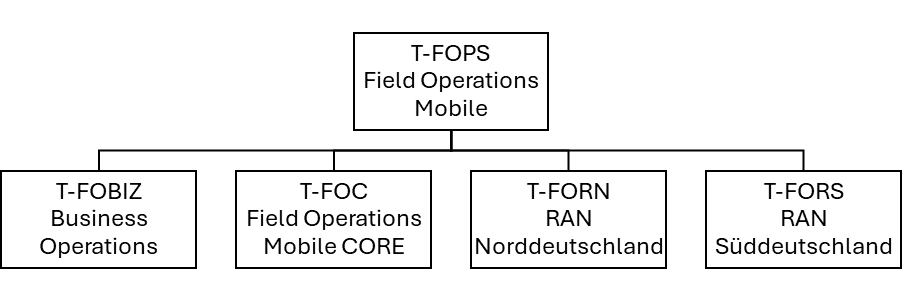
\includegraphics[width=0.7\textwidth]{abbildungen/FopsOrga}
    \caption{Organization Chart \ac{T-FOPS}}
    \label{fig:FopsOrga}
    source: own illustration
\end{figure}
\begin{figure}[H]
    \centering
    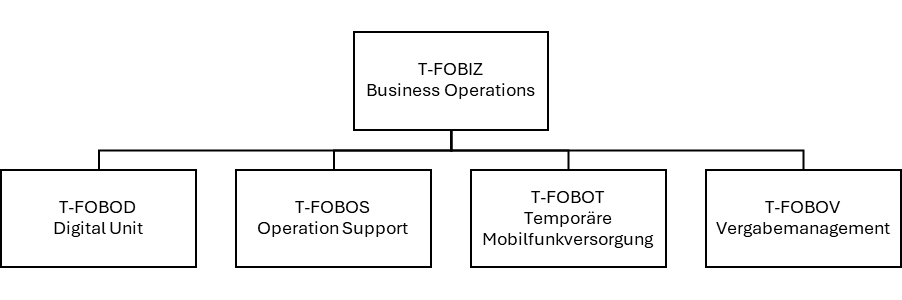
\includegraphics[width=0.7\textwidth]{abbildungen/FobizOrga}
    \caption{Organization Chart \ac{T-FOBIZ}}
    \label{fig:FobizOrga}
    source: own illustration
\end{figure}

\subsection{Structure of the Thesis}

\subsection{Scope and Limitations}


\newpage
\section{State of Research} 

\newpage
\section{Latex-Details} \label{latexDetails}

\subsection{Verwendete Software, Editor und Zusatzpakete}
\subsubsection{Windows 8+}
\begin{itemize}
\item MikTex: 2.9, 32-bit
\item Biblatex: 3.5, Zusatz: Biber.exe
\item Editor: TexStudio (kann ich empfehlen), Notepad++
\end{itemize}

\subsubsection{Mac OSX und iOS}
\begin{itemize}
\item MacTeX: \url{https://tug.org/mactex}
\item Editor: TexPad \url{https://www.texpadapp.com}
\end{itemize}

\subsubsection{Online}
Overleaf ist eine Online-Anwendung mit der Ihr direkt im Browser an eurer Thesis schreiben könnt. Bis 1GB Größe und maximal 60 Einzeldateien könnt ihr Overleaf kostenlos nutzen: \url{https://www.overleaf.com/}


\subsection{Dokumentenklasse}
Eigentlich hatte Prof. Finke empfohlen die Dokumentklassen \enquote{Book} oder \enquote{Report} für die Erstellung der Bachelor-Thesis zu verwenden, da diese über weitere Gliederungsebenen verfügen. Ich verwende dennoch eine leicht modifizierte Komaskript-Klasse \enquote{scrartcl}, mit der Erweiterung um eine Ebene. Siehe (skripte/weitereEbene.tex). Das Skript stammt irgendwo aus den Netz und übersteigt meine \LaTeX{}-Fähigkeiten. Dadurch kann ich über eine weitere Ebene in der Arbeit verfügen, ohne mich mit der Modifikation von Kapitel-Seiten rumschlagen~\footcite[Vgl. ][S. 5]{Tanenbaum.2003} zu müssen. Diese Quelle ist nur zur Demonstration und hat keinen inhaltlichen Bezug hierzu. Es werden übrigens nur die Quellen im Literaturverzeichnis angezeigt, die auch referenziert sind.


\subsection{Grafiken}
Das Paket \textbackslash usepackage\{float\} ermöglicht es die Grafiken und Tabellen an der Stelle im Text zu positionieren, wo diese im Quelltext stehen (Option H). Ansonsten würde \LaTeX{} diese dort unterbringen, wo es typographisch sinnvoll wäre - das wollen wir ja nicht ;-).

Die Breite der Grafiken am Besten relativ zum Text angeben.

\subsection{Quellcode}
Quellcode kann auf unterschiedliche Arten eingebaut werden.
Zum einen kann es hier durch direktives Einbinden in der Kapitel-Datei geschehen.
\begin{lstlisting}
% Hier wird aufgezeigt, wie man eine Grafik einbindet, es wird also in der PDF angezeigt,
% da es in einem Quellcode-Listing steht.
% Auch wenn es hier faelschlicherweise als LaTeX-Befehl angezeigt wird.
\includegraphics[width=0.9\textwidth]{sup}
\end{lstlisting}

Bei längeren Quellcode-Listings empfiehlt es sich jedoch auf eine externe Datei im Ordner Quellcode zu verlinken und diese einzubauen:
\lstinputlisting[language=HTML]{./Quellcode/Beispiel.html}

Statt dem Package lstlisting, welches direkt auf Tex basiert, kann auch das Package minted verwendet werden.
Dieses Package basiert auf python-pygments und unterstützt weit mehr Sprachkonstrukte als lstlisting.
Um das Paket zu verwenden muss es eingebunden werden und zusätzlich python-pygments installiert sein.
(Dies ist mit im Dockerfile vorhanden. Für die anderen Compile-Methoden, wie das native verwenden von Tex Live findet sich hier die Installationsanleitung für das minted Paket: https://ctan.org/pkg/minted?lang=de)

Damit das kompilieren ohne Python trotzdem möglich ist, ist die Funktion standardmäßig ausgebaut. Deshalb muss zusätzlich in der Datei \begin{verbatim}thesis_main.tex \usepackage{minted} \end{verbatim} wieder einkommentiert werden. 

Minted lässt sich dann ganz ähnlich zu lstlisting verwenden:
\begin{lstlisting}
	\begin{minted}{c}
		int main() {
			printf("hello, world");
			return 0;
		}
	\end{minted}
\end{lstlisting}	

Da der Pfad zu den Abbildungen im Hauptdokument definiert wurde, muss hier nur noch der Name des Bildes ohne Dateiendung stehen (sup).

\begin{figure}[H]
\caption{Titel der Abbildung hier}
\includegraphics[width=0.9\textwidth]{sup}
\\
Quelle: Eigene Darstellung
\end{figure}



%\clearpage % hiermit werden alle Bilder Tabellen ausgeworfen

\subsection{Biblatex}
\subsubsection{Erklärung}
Von den vielen verfügbaren Literatur-Paketen habe ich mich für Biblatex entschieden. Die Anforderungen der FOM sollten hiermit erfüllt sein. Ich habe bisher nur Einträge \enquote{@book} getestet. Wie immer steckt der Teufel hier im Detail und es wird sich später herausstellen, ob Biblatex eine gute Wahl war. Die Anpassungen hierfür liegen unter skripte/modsBiblatex. Ich verwende das Backend Biber, welches bib-Dateien in UTF-8 verarbeiten kann.

In der für den Leitfaden 2018 aktualisierten Version sind außerdem Beispiele für \enquote{online},\footcite[Vgl.][]{website:angular:aboutAngular} also Webseiten, und \enquote{article},\footcite[Vgl.][S. 140]{Decker2009} also wissenschaftliche Artikel, enthalten.

Laut Leitfaden sollen maximal 3 Autoren genannt werden und danach mit
\enquote{et. al.} bzw. \enquote{u.a.} ergänzt werden. Damit im Literaturverzeichnis auch nur max.
3 Autoren stehen, muss man beim Füllen der literatur.bib-Datei darauf achten auch nur 3
einzutragen. Weitere Autoren kann man einfach mit \enquote{and others} ergänzen.
Siehe Eintrag für \enquote{Balzert.2008}. Zitiert man dann diese Werk, werden auch in
der Fussnote alle Autoren korrekt genannt wie in dieser
Fußnote\footcite[Vgl.][S. 1]{Balzert.2008} zu sehen ist.

Hat man dagegen mehr als 3 Autoren in der bib-Datei hinterlegt, stehen im
Literaturverzeichnis alle drin. In der Fussnote dagegen, steht nur
einer\footcite[Vgl.][S. 1]{Balzert2.2008}, was dem Leitfaden widerspricht.

Die Anzahl von 3 wird übrigens über die Option \enquote{maxcitenames=3} des
biblatex-Packages gesetzt. Man muss selbst schauen, dass die Anzahl der Autoren
in den Bib-Dateien mit der Optionseinstellung übereinstimmt.

\subsubsection{Beispielfußnoten}
Diese Fussnote soll zeigen, wie mit einem \enquote{von} vor dem Namen des Autors
umgegangen wird\footcite[Vgl.][S. 1]{Lucke2018}. Man muss für die korrekte
Sortierung eines solchens Namens im Literaturverzeichnis einen \enquote{sortkey}
setzen.

Diese Fussnote soll zeigen, wie mit einer Online-Quelle ohne Jahresangabe
umgegangen wird\footcite[Vgl.][]{Belastingdienst}.

Diese Fußnote\footcite[Vgl.][S.1]{Beckert.2012} ist nur dazu da zu zeigen, wie mit mehreren Quellen des selben Autors aus dem selben Jahr umgegangen wird, wenn das Stichwort gleich bleibt \footcite[Vgl.][S.2]{Beckert.2012.1} oder sich ändert\footcite[Vgl.][S.3]{Beckert.2012.2}. Laut Leitfaden sollte bei gleichem Autor, Jahr und Stichwort ein Buchstabe an die Jahreszahl gehangen werden. Zum Beispiel 2012a. 

Die folgenden Fußnoten dienen dazu zu zeigen, dass die Nummern von zwei direkt aufeinanderfolgende Fußnoten mit Komma getrennt werden.\footcite[Vgl.][S.2]{Beckert.2012.1}\footcite[Vgl.][S. 1]{Lucke2018}
\subsection{Abkürzungen}
Abkürzungen werden mithilfe des Pakets Acronym eingebunden. Alle Abkürzungen sollten in der Datei acronyms.tex mithilfe des \begin{verbatim}
	\acro
\end{verbatim} Befehls festgelegt werden. Im Text werden diese dann mit \begin{verbatim}
	\ac{Abkürzung}
\end{verbatim} benutzt. Bei der ersten Verwendung einer Abkürzung wird der Begriff in beiden Formen dargestellt. So wie hier: \ac{WYSIWYG}. Nur wenn eine Abkürzung tatsächlich verwendet wird erscheint sie auch im Abkürzungsverzeichnis.

Sollte es im Abkürzungsverzeichnis zu Anzeigefehlern kommen kann dies daher rühren, dass eine Abkürzung verwendet wird, die länger ist als \ac{WYSIWYG}. In diesem Fall müsst ihr in der Datei acronyms.tex den Parameter [WYSIWYG] durch eure längere Abkürzung ersetzen.

\subsection{Formeln}
Um eine Formel nach links aus zurichten muss sie zwischen \& und \& eingesetzt werden:

\textbf{Formel 1: Erste Formel}
\begin{flalign}
   & L_P{=} 10lg \cdot \frac{P}{1 mW} &
\end{flalign}
\cite[Quelle: In Anlehnung an][S. 4]{Beckert.2012}


Etwas mehr Text.

Ansonsten wird sie mittig ausgerichtet test.
% Mehr infos: http://www.ctex.org/documents/packages/math/amsldoc.pdf

\textbf{Formel 2: Zweite Formel}
\begin{flalign}
   L_P{=} 10lg \cdot \frac{P}{1 mW}
\end{flalign}
\cite[Quelle: In Anlehnung an][S. 4]{Beckert.2012}

\subsection{Symbole}
% die folgenden Symbole haben nicht mit der Formel oben drüber zu tun
Das hier ist ein definiertes Symbol: \symnz und das hier auch \AB . Symbole werden in der Datei Skripte symboldef.tex zentral definiert.

\subsection{Glossar}
Begriffserklärungen bzw. das \gls{glossar} wird mithilfe des Pakets \gls{glossaries} eingebunden. Alle Begriffe die erklärt werden sollen, sollten in der Datei glossar.tex mithilfe des \begin{verbatim}
	\newglossaryentry
\end{verbatim} Befehls festgelegt werden. Im Text werden diese dann mit \begin{verbatim}
	\gls{Begriff}
\end{verbatim} benutzt.


\subsection{Listen und Aufzählungen}
\subsubsection{Listen}
\begin{itemize}
\item ein wichtiger Punkt
\item noch ein wichtiger Punkt
\item und so weiter
\end{itemize}
\subsubsection{Aufzählungen}
\begin{enumerate}
\item Reihenfolge ist hier wichtig
\item Dieser Punkt kommt nach dem ersten
\item Da sollte jetzt eine 3 vorne stehen
\end{enumerate}

\paragraph{Tiefste Ebene 1}
Dies ist die tiefste Gliederungsebene. Sollten doch mehr Ebenen benötigt werden, muss eine andere Dokumentenklasse verwendet werden.

\paragraph{Tiefste Ebene 2}
Der zweite Punkt in dieser Ebene ist zur Erinnerung daran, dass es nie nie niemals nur einen Unterpunkt geben darf.

\subsection{Skript zum Kompilieren}
Latex will ja bekanntlich in einer bestimmten Reihenfolge aufgerufen werden:
\begin{lstlisting}
lualatex thesis_main.tex
biber thesis_main
lualatex thesis_main.tex
lualatex thesis_main.tex
thesis_main.pdf
\end{lstlisting}

Dies ist der Inhalt der Batchdatei \enquote{compile.bat}.

\subsection{PlantUML}

\begin{lstlisting}
\begin{plantuml}
@startuml
Class01 <|-- Class02
Class03 *-- Class04
Class05 o-- Class06
Class07 .. Class08
Class09 -- Class10
@enduml
\end{plantuml}
\end{lstlisting}

\newpage
\section{Implementation}
\subsection{Requirements Engineering}
\subsection{...}
\subsection{Testing}

\newpage
\section{Evaluation}



\newpage
\section{Conclusion and Outlook}

\newpage
\section{Kritischer Ausblick und Fazit}



%-----------------------------------
% Apendix / Anhang
%-----------------------------------
%\newpage
%\section*{\AppendixName} %Überschrift "Anhang", ohne Nummerierung
%\addcontentsline{toc}{section}{\AppendixName} %Den Anhang ohne Nummer zum Inhaltsverzeichnis hinzufügen

%\begin{appendices}
% Nachfolgende Änderungen erfolgten aufgrund von Issue 163
%\makeatletter
%\renewcommand\@seccntformat[1]{\csname the#1\endcsname:\quad}
%\makeatother
%\addtocontents{toc}{\protect\setcounter{tocdepth}{0}} %
%\renewcommand{\thesection}{\AppendixName\ \arabic{section}}
%\renewcommand\thesubsection{\AppendixName\ \arabic{section}.\arabic{subsection}}
%\section{Beispielanhang}\label{Beispielanhang}
Dieser Abschnitt dient nur dazu zu demonstrieren, wie ein Anhang aufgebaut seien kann.
\subsection{Weitere Gliederungsebene}
Auch eine zweite Gliederungsebene ist möglich.
\section{Bilder}
Auch mit Bildern.
Diese tauchen nicht im Abbildungsverzeichnis auf.

%\end{appendices}
%\addtocontents{toc}{\protect\setcounter{tocdepth}{2}}

%-----------------------------------
% Literaturverzeichnis
%-----------------------------------
\newpage

% Die folgende Zeile trägt ALLE Werke aus literatur.bib in das
% Literaturverzeichnis ein, egal ob sie zietiert wurden oder nicht.
% Der Befehl ist also nur zum Test der Skripte sinnvoll und muss bei echten
% Arbeiten entfernt werden.
%\nocite{*}
\phantomsection
\addcontentsline{toc}{section}{Bibliography}

% Die folgenden beiden Befehle würden ab dem Literaturverzeichnis wieder eine
% römische Seitennummerierung nutzen.
% Das ist nach dem Leitfaden nicht zu tun. Dort steht nur dass 'sämtliche
% Verzeichnisse VOR dem Textteil' römisch zu nummerieren sind. (vgl. S. 3)
%\pagenumbering{Roman} %Zähler wieder römisch ausgeben
%\setcounter{page}{4}  %Zähler manuell hochsetzen

% Ausgabe des Literaturverzeichnisses

% Keine Trennlinie zwischen den einzelnen Einträgen
\renewcommand{\bibliography}[1]{\printbibliography}

%\bibliography{literatur/literatur}
\printbibliography[title=Literaturverzeichnis]
\addtocontents{toc}{\protect\newpage} %Eine neue Seite für die Versicherung

\newpage
\pagenumbering{gobble} % Keine Seitenzahlen mehr

%-----------------------------------
% Ehrenwörtliche Erklärung
%-----------------------------------
\section *{%
	\langen{Reference of AI Tools}}
	\langen{I hereby declare that I have used the following AI tools for this thesis:} \\
	\langen{•⁠  ⁠DeepL for translating parts of the thesis from German to English} \\
	\langen{•⁠  ⁠GitHub Copilot for code suggestions and completions for the LaTeX code \\• OpenAI ChatGPT for supporting the brainstorming ideas for the thesis}


\section*{%
	\langde{Ehrenwörtliche Erklärung}
	\langen{Declaration in lieu of oath}}
\langde{Hiermit versichere ich, dass die vorliegende Arbeit von mir selbstständig und ohne unerlaubte Hilfe angefertigt worden ist, insbesondere dass ich alle Stellen, die wörtlich oder annähernd wörtlich aus Veröffentlichungen entnommen sind, durch Zitate als solche gekennzeichnet habe. Ich versichere auch, dass die von mir eingereichte schriftliche Version mit der digitalen Version übereinstimmt. Weiterhin erkläre ich, dass die Arbeit in gleicher oder ähnlicher Form noch keiner Prüfungsbehörde/Prüfungsstelle vorgelegen hat. Ich erkläre mich damit \textcolor{red}{einverstanden}, dass die Arbeit der Öffentlichkeit zugänglich gemacht wird. Ich erkläre mich damit einverstanden, dass die Digitalversion dieser Arbeit zwecks Plagiatsprüfung auf die Server externer Anbieter hochgeladen werden darf. Die Plagiatsprüfung stellt keine Zurverfügungstellung für die Öffentlichkeit dar.}
\langen{I hereby declare that I produced the submitted paper with no assistance from any other party and without the use of any unauthorized aids and, in particular, that I have marked as quotations all passages which are reproduced verbatim or near-verbatim from publications. Also, I declare that the submitted print version of this thesis is identical with its digital version. Further, I declare that this thesis has never been submitted before to any examination board in either its present form or in any other similar version. I herewith \textcolor{red}{agree} that this thesis may be published. I herewith consent that this thesis may be uploaded to the server of external contractors for the purpose of submitting it to the contractors’ plagiarism detection systems. Uploading this thesis for the purpose of submitting it to plagiarism detection systems is not a form of publication.}


\par\medskip
\par\medskip

\vspace{5cm}

\begin{table}[H]
	\centering
	\begin{tabular*}{\textwidth}{c @{\extracolsep{\fill}} ccccc}
		\myOrt, \the\day.\the\month.\the\year
		&
		% Hinterlege deine eingescannte Unterschrift im Verzeichnis /abbildungen und nenne sie unterschrift.png
		% Bilder mit transparentem Hintergrund können teils zu Problemen führen
		
\includegraphics[width=0.6\textwidth]{unterschrift}\vspace*{-0.6cm}
		\\
		\rule[0.5ex]{12em}{0.55pt} & \rule[0.5ex]{12em}{0.55pt} \\
		\langde{(Ort, Datum)}\langen{(Location, Date)} & \langde{(Eigenhändige Unterschrift)}\langen{(handwritten signature)}
		\\
	\end{tabular*} \\
\end{table}


\end{document}